% chapters/results.tex
\chapter{Results}
\label{ch:results}

This chapter presents the empirical findings in three parts: AHP criterion weights
and reliability checks, per-model Likert scores, and the final interval-based
ranking.

% ---------------------------------------------------------------
\section{AHP Consistency and Criterion Weights}
\label{sec:res-ahp}

\subsection{Consistency Analysis}
\label{subsec:res-consistency}

Ten reviewers provided pairwise comparison matrices. Table~\ref{tab:cr} reports the
principal eigenvalue $\lambda_{\max}$, the Consistency Index (CI), the Consistency
Ratio (CR), and the resulting status for each judge. Judges with $\mathrm{CR} > 0.10$
are excluded from weight derivation.

\begin{table}[H]
  \centering
  \caption{AHP consistency analysis for all judges. Judges marked \emph{Consistent}
    ($\mathrm{CR} < 0.10$) are retained for criterion weight derivation.}
  \label{tab:cr}
  \begin{tabular}{lcccc}
    \toprule
    Judge & $\lambda_{\max}$ & CI & CR & Status \\
    \midrule
    J1  & 4.1057 & 0.0352 & 0.0315 & Consistent \\
    J2  & 4.3094 & 0.1031 & 0.0921 & Consistent \\
    J3  & 4.2198 & 0.0733 & 0.0654 & Consistent \\
    J4  & 5.4383 & 0.4794 & 0.4281 & Inconsistent \\
    J5  & 4.7165 & 0.2388 & 0.2132 & Inconsistent \\
    J6  & 4.4892 & 0.1631 & 0.1456 & Inconsistent \\
    J7  & 5.7219 & 0.5740 & 0.5125 & Inconsistent \\
    J8  & 4.1427 & 0.0476 & 0.0425 & Consistent \\
    J9  & 5.1200 & 0.3733 & 0.3333 & Inconsistent \\
    J10 & 5.6719 & 0.5573 & 0.4976 & Inconsistent \\
    \bottomrule
  \end{tabular}
\end{table}

Four judges (J1, J2, J3, J8) satisfy the consistency requirement. Their weights are
aggregated using a CR-weighted geometric mean, so that more consistent judges exert
greater influence on the final weights.

\subsection{Criterion Priorities}
\label{subsec:res-weights}

Table~\ref{tab:weights-main} reports the major-criterion priorities, and
Tables~\ref{tab:weights-sub1}--\ref{tab:weights-sub4} report sub-criterion
priorities within each major criterion.

\begin{table}[H]
  \centering
  \caption{AHP major-criterion priorities under CR weighting.}
  \label{tab:weights-main}
  \begin{tabular}{lcc}
    \toprule
    Criterion & Priority & Percentage \\
    \midrule
    Trustworthiness (C4)   & 0.4565 & 45.65\% \\
    Completeness (C2)      & 0.3053 & 30.53\% \\
    Usefulness (C3)        & 0.1260 & 12.60\% \\
    Understandability (C1) & 0.1121 & 11.21\% \\
    \bottomrule
  \end{tabular}
\end{table}

\begin{table}[H]
  \centering
  \caption{Sub-criterion priorities: Understandability (C1).}
  \label{tab:weights-sub1}
  \begin{tabular}{lc}
    \toprule
    Sub-Criterion & Priority \\
    \midrule
    S1.1 — Clarity           & 0.7192 \\
    S1.2 — Ease of Following & 0.2808 \\
    \bottomrule
  \end{tabular}
\end{table}

\begin{table}[H]
  \centering
  \caption{Sub-criterion priorities: Completeness (C2).}
  \label{tab:weights-sub2}
  \begin{tabular}{lc}
    \toprule
    Sub-Criterion & Priority \\
    \midrule
    S2.1 — Coverage        & 0.5708 \\
    S2.2 — Reasoning Depth & 0.4292 \\
    \bottomrule
  \end{tabular}
\end{table}

\begin{table}[H]
  \centering
  \caption{Sub-criterion priorities: Usefulness (C3).}
  \label{tab:weights-sub3}
  \begin{tabular}{lc}
    \toprule
    Sub-Criterion & Priority \\
    \midrule
    S3.1 — Goal Support                       & 0.4767 \\
    S3.2 — Decision-Making / Error Prevention & 0.5233 \\
    \bottomrule
  \end{tabular}
\end{table}

\begin{table}[H]
  \centering
  \caption{Sub-criterion priorities: Trustworthiness (C4).}
  \label{tab:weights-sub4}
  \begin{tabular}{lc}
    \toprule
    Sub-Criterion & Priority \\
    \midrule
    S4.1 — Reliability         & 0.7108 \\
    S4.2 — Alignment \& Safety & 0.2892 \\
    \bottomrule
  \end{tabular}
\end{table}

Trustworthiness receives the highest weight at 45.65\%, followed by Completeness at
30.53\%. Together these two criteria account for over 75\% of total weight,
confirming that students prioritise causal integrity over surface fluency. Among
sub-criteria, Clarity (S1.1) and Reliability (S4.1) emerge as the dominant factors
within their respective major criteria.

% ---------------------------------------------------------------
\section{Inter-Rater Reliability}
\label{sec:res-reliability}

Three reliability analyses were applied to the full set of 2{,}592 Likert responses.

\begin{itemize}
  \item \textbf{Intraclass Correlation:} $\mathrm{ICC}(2,k) = 0.780$, indicating
    consistent ratings across reviewers and exceeding the 0.60 threshold required for
    aggregation validity.
  \item \textbf{Krippendorff's $\alpha$:} $\alpha = 0.757$ (interval scale),
    supporting substantial agreement among raters \citep{hayes2007answering}.
  \item \textbf{Effect sizes:} When comparing the top model (\texttt{qwen2.5:14b})
    against the lowest (\texttt{phi3:3.8b}), Cohen's $d$ and Hedges' $g$ both
    indicate a large effect, confirming that score differences are practically
    meaningful.
\end{itemize}

Both ICC and Krippendorff's $\alpha$ exceed their respective thresholds, validating
the aggregation procedure.

% ---------------------------------------------------------------
\section{LLM Performance on Human Ratings}
\label{sec:res-models}

Figures~\ref{fig:radar-qwen14b}--\ref{fig:radar-codellama} show the radar charts for
all nine models, each plotting the four evaluation criteria (Understandability,
Completeness, Usefulness, Trustworthiness) across the five reasoning task categories
(Academic Knowledge, Procedural Knowledge, Problem Solving Ability, Qualitative
Reasoning, Quantitative Reasoning). The shaded area represents the IQR interval for
each dimension, making reviewer disagreement directly visible. All radar charts are
generated by \texttt{code/E2\_AHP\_CSV\_AND\_GRAPHS.ipynb}.

\begin{figure}[H]
  \centering
  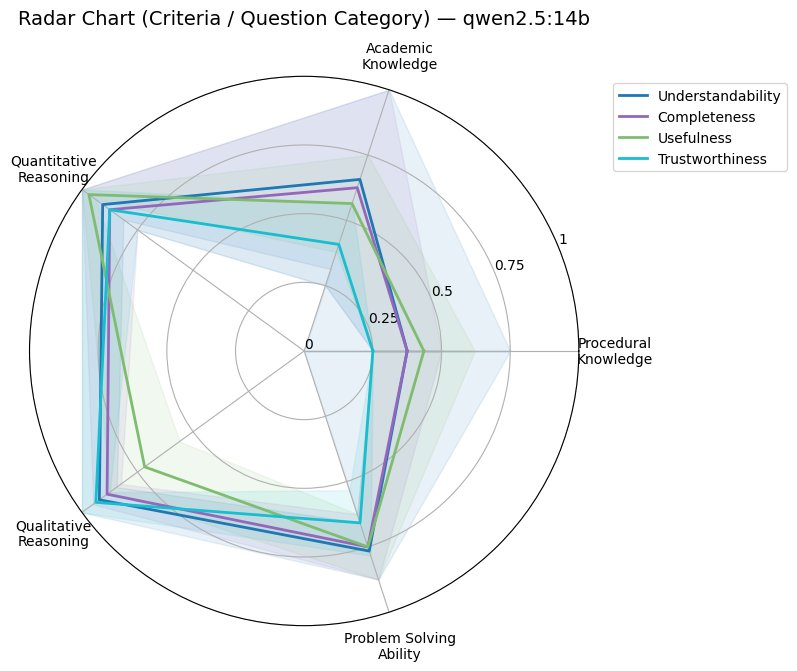
\includegraphics[width=0.78\textwidth]{figures/qwen2_5_14b.png}
  \caption{Radar chart for \texttt{qwen2.5:14b}. The model covers all five reasoning
    categories with the largest and most balanced polygon, indicating strong
    performance across all four criteria. IQR bands are narrow, reflecting reviewer
    consensus.}
  \label{fig:radar-qwen14b}
\end{figure}

\begin{figure}[H]
  \centering
  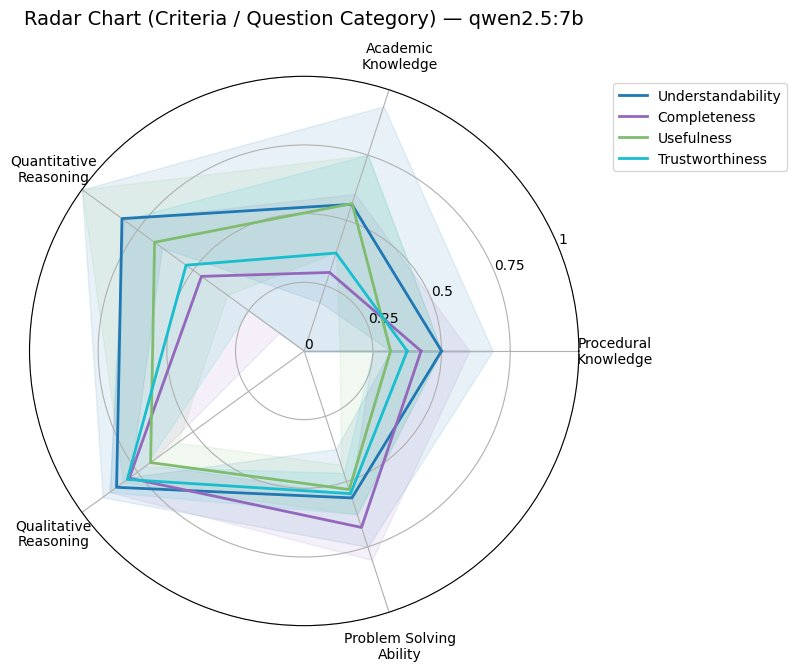
\includegraphics[width=0.78\textwidth]{figures/qwen2_5_7b.png}
  \caption{Radar chart for \texttt{qwen2.5:7b}. Performance is somewhat below the
    14B variant, particularly in Quantitative Reasoning, but the model forms a
    strong second tier.}
  \label{fig:radar-qwen7b}
\end{figure}

\begin{figure}[H]
  \centering
  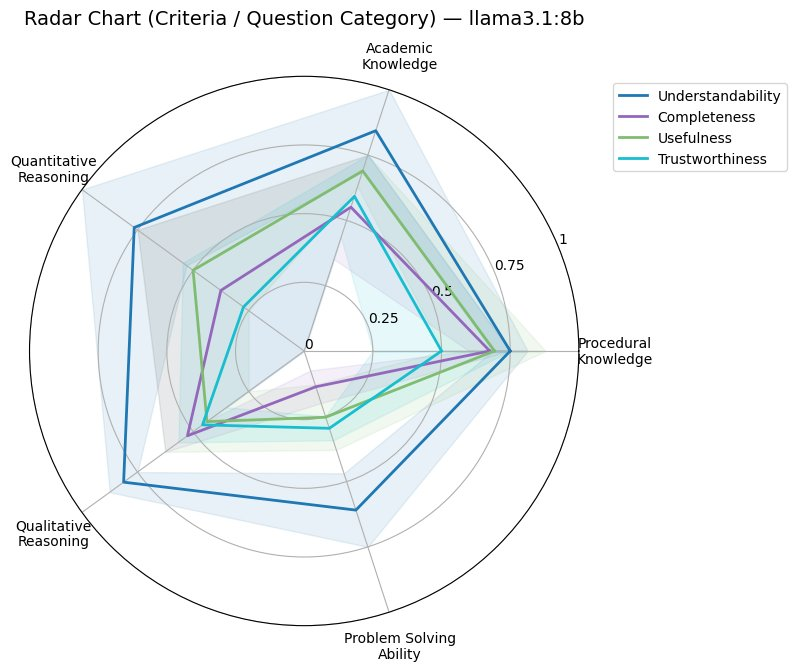
\includegraphics[width=0.78\textwidth]{figures/llama3_1_8b.png}
  \caption{Radar chart for \texttt{llama3.1:8b}. The model is strongest in Academic
    Knowledge and weakest in Procedural tasks, showing complementary strengths to
    Mistral-Nemo.}
  \label{fig:radar-llama}
\end{figure}

\begin{figure}[H]
  \centering
  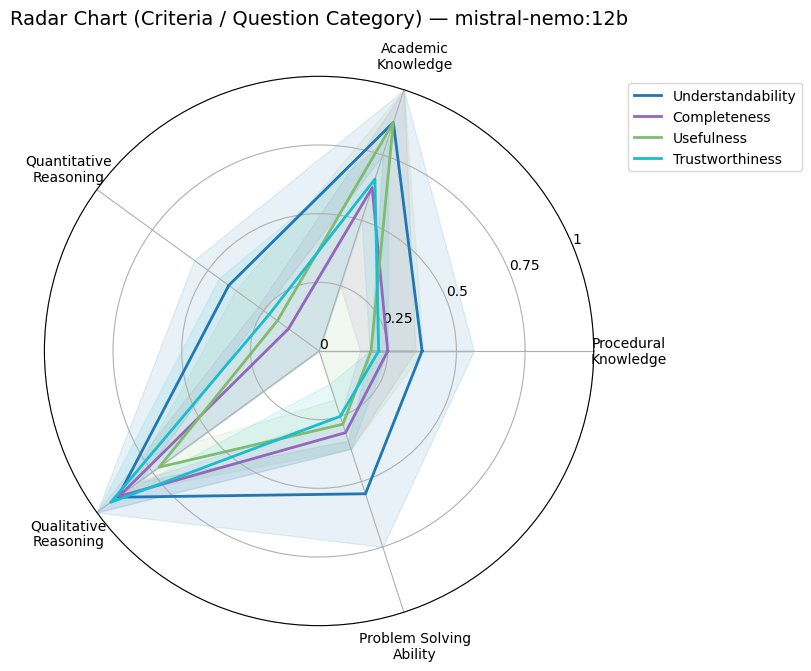
\includegraphics[width=0.78\textwidth]{figures/mistral-nemo_12b.png}
  \caption{Radar chart for \texttt{mistral-nemo:12b}. The model leads on Academic
    Knowledge but struggles on Procedural tasks. Large IQR bands in Quantitative
    Reasoning indicate reviewer disagreement.}
  \label{fig:radar-nemo}
\end{figure}

\begin{figure}[H]
  \centering
  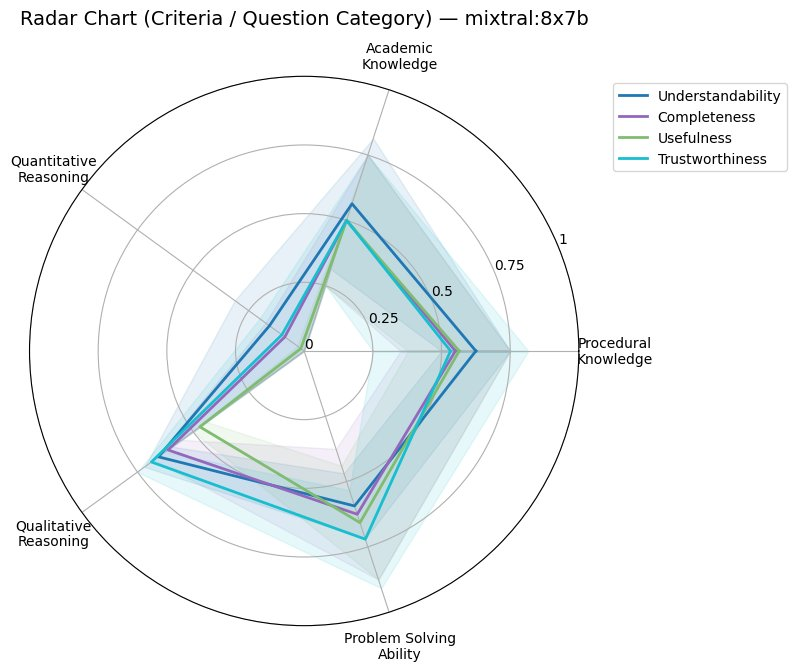
\includegraphics[width=0.78\textwidth]{figures/mixtral_8x7b.png}
  \caption{Radar chart for \texttt{mixtral:8x7b}. Performance is balanced across
    categories, with a relative strength in Procedural Knowledge.}
  \label{fig:radar-mixtral}
\end{figure}

\begin{figure}[H]
  \centering
  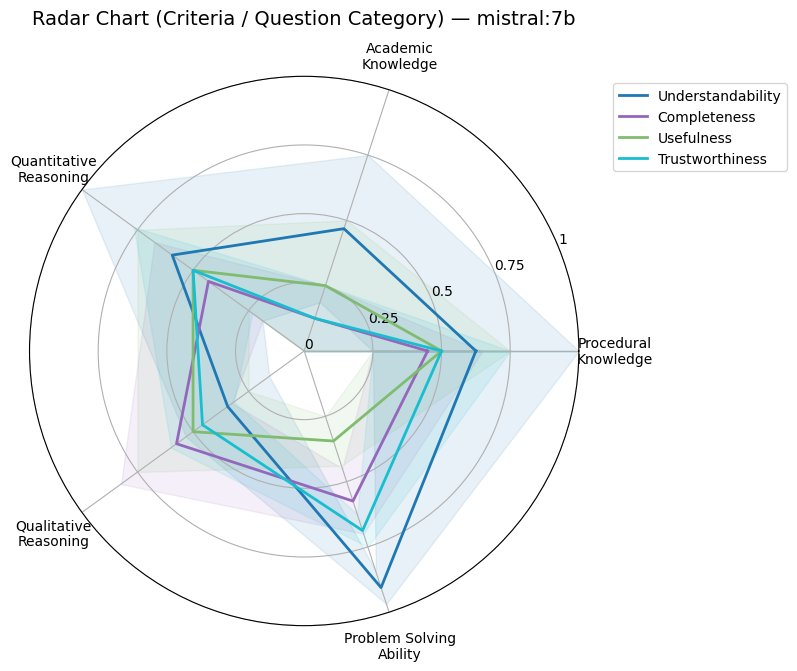
\includegraphics[width=0.78\textwidth]{figures/mistral_7b.png}
  \caption{Radar chart for \texttt{mistral:7b}. The model illustrates the
    fluency trap: Understandability scores are relatively high (0.552) while
    Trustworthiness scores are markedly lower (0.428), indicating that surface
    coherence does not reflect causal reliability.}
  \label{fig:radar-mistral7b}
\end{figure}

\begin{figure}[H]
  \centering
  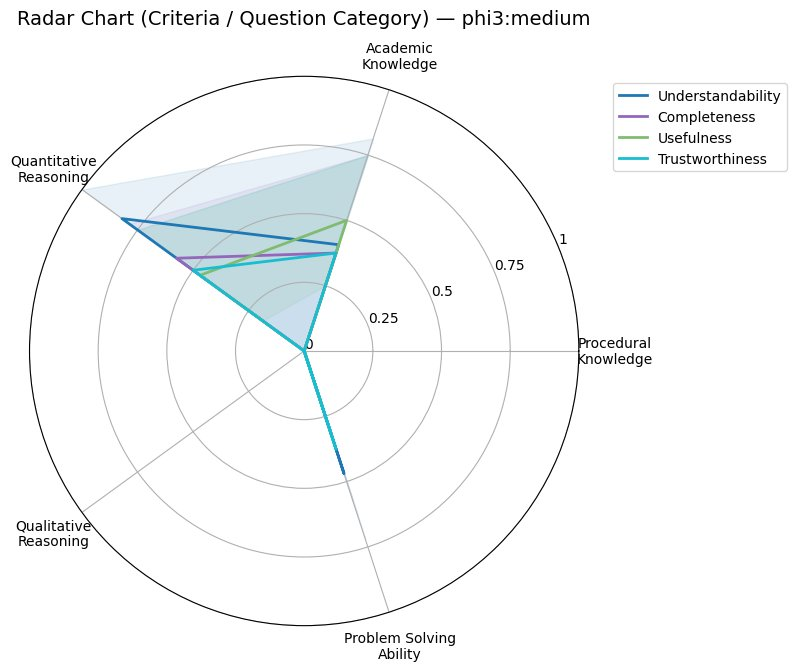
\includegraphics[width=0.78\textwidth]{figures/phi3_medium.png}
  \caption{Radar chart for \texttt{phi3:medium}. Performance is restricted
    primarily to the Academic Knowledge and Quantitative Reasoning axes, with
    near-zero scores elsewhere.}
  \label{fig:radar-phi3m}
\end{figure}

\begin{figure}[H]
  \centering
  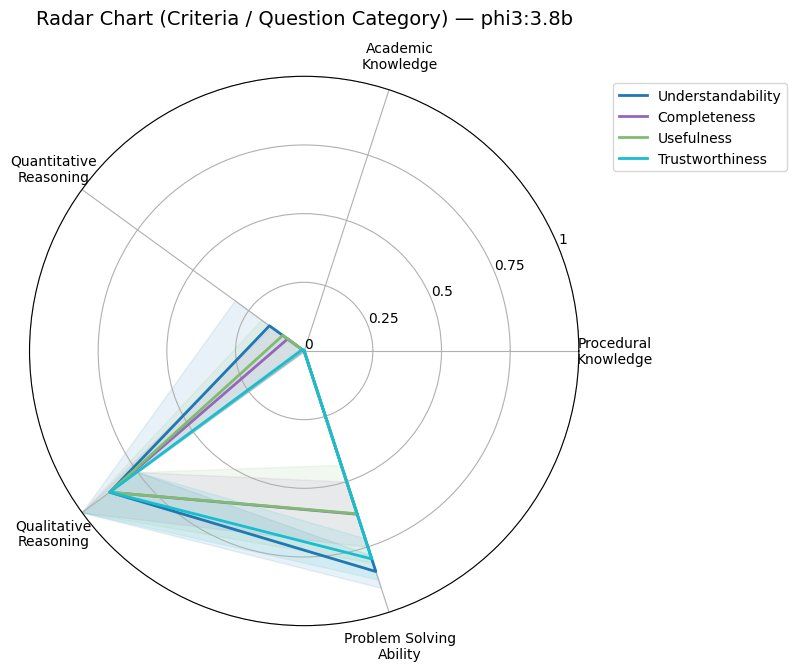
\includegraphics[width=0.78\textwidth]{figures/phi3_3_8b.png}
  \caption{Radar chart for \texttt{phi3:3.8b}. Scores cluster in the lower
    portion of the chart. The model ranks last overall. Notably, within the Phi
    family, the smaller 3.8B model outperforms the larger Medium variant,
    indicating that architecture matters more than parameter count.}
  \label{fig:radar-phi3s}
\end{figure}

\begin{figure}[H]
  \centering
  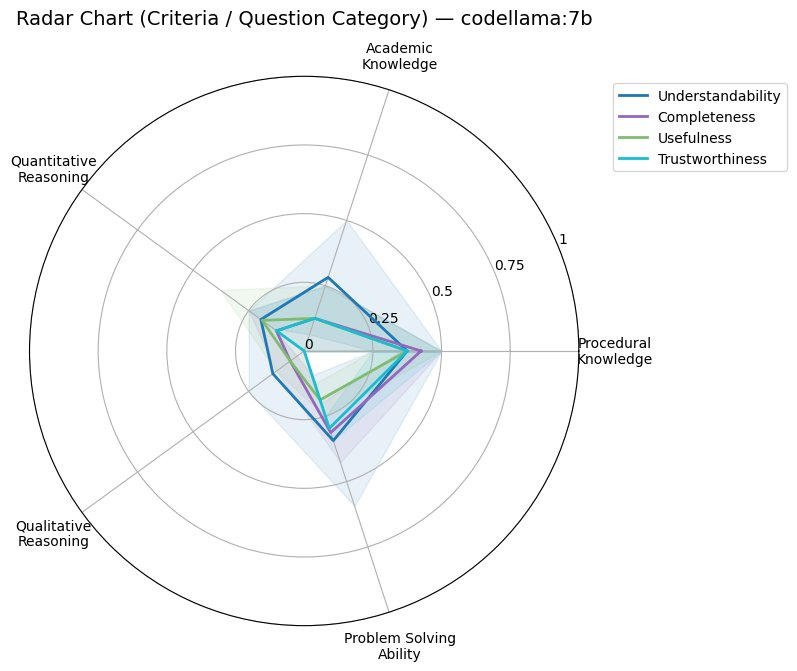
\includegraphics[width=0.78\textwidth]{figures/codellama_7b.png}
  \caption{Radar chart for \texttt{codellama:7b}. The weakest overall model,
    especially in Trustworthiness and Qualitative Reasoning. The polygon covers
    a minimal area.}
  \label{fig:radar-codellama}
\end{figure}

\subsection{Summary of Model Performance Patterns}
\label{subsec:res-patterns}

Three main patterns emerge from the human ratings.

First, \texttt{qwen2.5:14b} achieves the highest scores across all criteria and
question categories. It is the most balanced model, with particular strength in
Academic Knowledge and Problem Solving Ability. Its narrow IQR bands indicate that
reviewer judgments are consistent, i.e., the model produces stable and interpretable
explanations.

Second, \texttt{qwen2.5:7b} and \texttt{llama3.1:8b} form a strong second tier.
They perform well in completeness and usefulness, though slightly below the 14B
Qwen model in trustworthiness. Parameter scaling within the Qwen family from 7B to
14B raises the performance floor by approximately 76\%, indicating that scaling
reduces severe reasoning failures.

Third, \texttt{codellama:7b} and \texttt{phi3:3.8b} score lowest across most
criteria, with averages near or below 2.0 on the 5-point Likert scale. These models
do not meet the baseline reliability threshold required for reviewers to evaluate
secondary qualities such as completeness or usefulness.

A recurring fluency trap is observed most clearly in \texttt{mistral:7b}: the model
scores high on Understandability but substantially lower on Trustworthiness,
suggesting that linguistically coherent outputs can mask causally unreliable
reasoning. This pattern is pedagogically significant because students may misplace
trust in fluent but flawed explanations.

Interval width varies systematically across question categories. It is highest for
Quantitative and Procedural Reasoning tasks, where distinguishing valid causal steps
from plausible narratives is most difficult, and narrowest for Qualitative Reasoning,
where reviewer consensus is strongest.

% ---------------------------------------------------------------
\section{Adaptive Question Selection: Impact Assessment}
\label{sec:res-qselect}

The MAD-style selection procedure identified 12 questions from the 140-item MMLU
Economics subset that maximise both internal model disagreement and external
diversity relative to each other. These questions produced high variance in human
judgments. For example, questions covering moving average processes and aggregate
demand showed strong structural divergence across models, with some models providing
complete stepwise causal chains while others generated incomplete or generic
explanations. The selection procedure reduces the annotation burden by 91\%
(from 3{,}780 to 324 assessments) while ensuring that the selected items cover
distinct regions of the explanation space \citep{feng2025sample}.
